%%%%%%%%%%%%%%%%%%%%%%%%%%%%%%%%%%%%%%%%%%%%%%%%%%%%%%%%%%%%%%%%%%%%%%
% CS624: Analysis of Algorithms
% Copyright 2015 Pejman Ghorbanzade <mail@ghorbanzade.com>
% Creative Commons Attribution-ShareAlike 4.0 International License
% More info: https://bitbucket.org/ghorbanzade/umb-cs624-2015s
%%%%%%%%%%%%%%%%%%%%%%%%%%%%%%%%%%%%%%%%%%%%%%%%%%%%%%%%%%%%%%%%%%%%%%

\section*{Question 7}

Suppose $n = 16$. Draw the recursion tree for Equation \ref{eq16}, including every node in the tree. Since $n$ is finite, there are only a finite number of nodes in the tree. You need to show every one of them.

\begin{equation}
T(n) = T(\frac{n}{4})+T(\frac{n}{2})+n^2
\label{eq16}
\end{equation}

\subsection*{Solution}

Recursion tree for Equation \ref{eq16} is depicted in Figure \ref{fig1}.

\begin{figure}[H]\centering
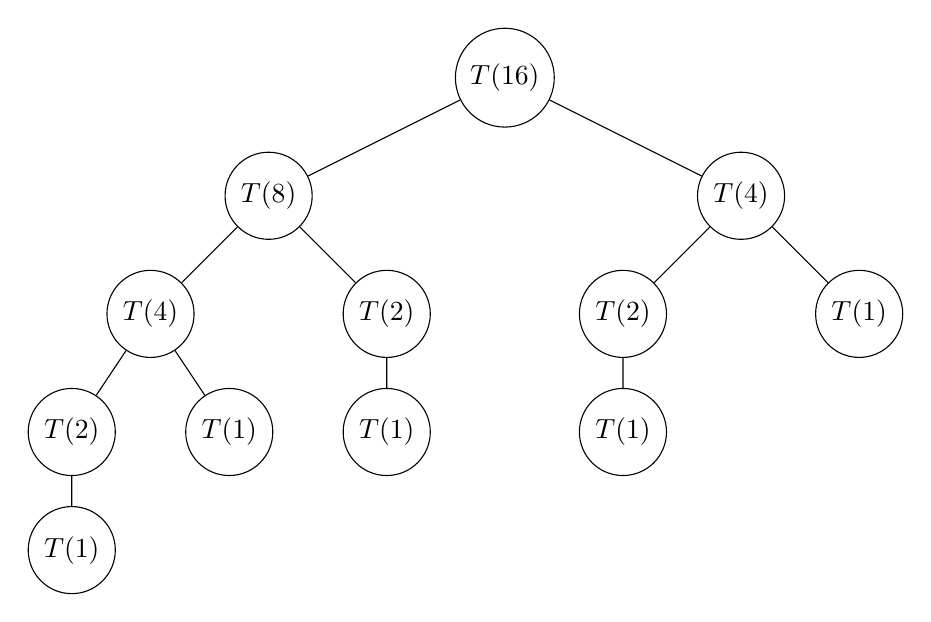
\begin{tikzpicture}[level/.style={sibling distance=60mm/#1}]
\node [circle,draw] (z){$T(16)$}
  child {
    node [circle,draw] (a) {$T(8)$}
    child {
      node [circle,draw] (c) {$T(4)$}
      child {
        node [circle,draw] (g) {$T(2)$}
        child {
          node [circle,draw] (k) {$T(1)$}
        }
      }
      child {
        node [circle,draw] (h) {$T(1)$}
      }
    }
    child {
      node [circle,draw] (d) {$T(2)$}
      child {
        node [circle,draw] (i) {$T(1)$}
      }
    }
  }
  child {
    node [circle,draw] (b) {$T(4)$}
    child {
      node [circle,draw] (e) {$T(2)$}
      child {
        node [circle,draw] (j) {$T(1)$}
      }
    }
    child {
      node [circle,draw] (f) {$T(1)$}
    }
  };
\end{tikzpicture}
\caption{Recursion tree for $T(n)=T(\frac{n}{2})+T(\frac{n}{4})+n^2$ when $n = 16$}\label{fig1}
\end{figure}
